% Compile twice from this directory:
%   pdflatex r2_reviewreport.tex
\documentclass{ssnreview}
\usepackage{amsmath}
\usepackage{amsfonts}
\usetikzlibrary{positioning}

\projecttitle{PAYLOAD-AWARE TWO-TIER UAV ROUTE PLANNING FOR LAST-MILE DELIVERY}
\reviewnumber{REVIEW REPORT -- II}
\students{%
  Thirumurugan RA (3122235001149)\\
  Meghna Manimaran (3122235001079)\\
  Shrika SP Thota (3122235001125)}
\supervisor{Dr. N. Sujaudeen, Assistant Professor}
\department{Department of Computer Science and Engineering}
\institution{Sri Sivasubramaniya Nadar College of Engineering}
\academicyear{2026--2027}
\collegelogo{ssn-logo.png}

\newcommand{\tagtuple}{(F,W,U,P)}
\newcommand{\riskweight}{w_{\mathrm{risk}}}
\newcommand{\distweight}{w_{\mathrm{distance}}}
\newcommand{\energyweight}{w_{\mathrm{energy}}}

\begin{document}
\makereviewtitle
\reviewfrontmatter

\begin{reviewabstract}
Last-mile UAV delivery has to balance flight distance, energy consumption and route risk. A single shortest path is
not suitable for all delivery missions: a fragile medical payload should prefer safer corridors, while an urgent
payload should prefer shorter travel time where the risk is acceptable. The project therefore uses a two-tier
planner. Tier 1 constructs a reusable Pareto front of non-dominated routes for a delivery region. Tier 2 reads the
payload tags and selects one route from that front using a deterministic payload-aware scoring rule. This separates
regional route generation from mission-specific selection and avoids manual weight retuning for every delivery.

For Review 2, the implementation has been extended beyond the initial synthetic demonstration. The current codebase
contains a graph builder, NAMOA* Tier 1 engine, baseline algorithms, Tier 2 selector with validation and mission
export support, evaluation helpers, a benchmark smoke path, and a minimal operator dashboard. The Review 2 report
documents those modules, the revised payload tag schema, the first-review changes, and the current validation status.
The available results are from offline tests and generated fixtures unless explicitly marked otherwise; live OSM,
weather, DEM, Mission Planner, QGroundControl, SITL and hardware validation remain limitations for the next stage.

\keywords{UAV route planning; Pareto front; payload-aware selection; NAMOA*; last-mile delivery}
\end{reviewabstract}

\chapter{Introduction and Objectives}
Unmanned aerial vehicles can shorten last-mile delivery in dense urban regions, but the planner must respect multiple
conflicting objectives. A route with minimum distance can pass near dense buildings or no-fly regions. A low-risk
route can be longer and drain more battery. An energy-saving route can be unsuitable for urgent delivery. The project
addresses this trade-off for small UAV delivery missions by using a two-tier planning architecture.

Tier 1 builds a region-level Pareto front over three objectives: distance, energy and risk. Tier 2 uses mission
metadata to choose one route from that front. The mission metadata is encoded as four operator tags:
\begin{itemize}
  \item Fragility class, \(F \in \{1,\ldots,5\}\), which increases the risk weight.
  \item Payload weight class, \(W \in \{1,\ldots,3\}\), which increases the energy weight.\footnote{The frozen
  abstract used the term ``temperature sensitivity''. The current implementation uses payload weight class \(W\)
  because payload mass directly affects energy use.}
  \item Urgency class, \(U \in \{1,\ldots,3\}\), which increases the distance weight.
  \item Priority class, \(P \in \{1,\ldots,5\}\), which amplifies the dominant requirement for high-priority cases.
\end{itemize}

\section{Objectives}
\begin{enumerate}[label=\arabic*.]
  \item Build a reusable airspace graph and Pareto front for a delivery region.
  \item Select a route from the front using the payload tag tuple \(\tagtuple\), without manual weight retuning.
  \item Compare the proposed Tier 1 front and Tier 2 selector against baseline route choices.
  \item Export a selected route into a mission format suitable for later ground-station validation.
  \item Report the current validation honestly, separating offline fixture results from live or hardware validation.
\end{enumerate}

\chapter{First Review - Queries and Answers}
The first review clarified the novelty and changed the design from an extreme-point rule into a full Pareto-front
selection rule. Table~\ref{tab:first-review} summarises the main queries and their resolution in the current design.

\begin{table}[H]
\centering
\caption{First review queries and current resolution}
\label{tab:first-review}
\begin{tabularx}{\textwidth}{p{0.31\textwidth}X}
\toprule
\textbf{Review query} & \textbf{Resolution in current work} \\
\midrule
How are Tier 1 objectives connected to Tier 2 payload factors? &
Tier 2 derives objective weights directly from \(\tagtuple\). Fragility maps to risk, payload weight maps to
energy, and urgency maps to distance. \\
\addlinespace
Does Tier 2 only choose obvious extreme routes? &
No. The selector scores every route in the Pareto front and can select non-extreme points. The evaluation code
records point type, objective ranks and non-extreme selections. \\
\addlinespace
Why not use one fixed weighted sum before search? &
A fixed scalarisation gives the same trade-off for all missions and can miss unsupported Pareto points. The proposed
method builds the front once and changes only the mission-specific selection step. \\
\addlinespace
How will the route be used by an operator? &
The current integration adds a minimal dashboard and QGroundControl/Mission Planner waypoint export. SITL and real
ground-station loading are documented as pending validation. \\
\bottomrule
\end{tabularx}
\end{table}

\chapter{Problem Statement}
Given an airspace graph \(G=(V,E)\), a source node \(s\), a target node \(t\), and a payload tag tuple
\(\tagtuple\), the task is to choose one route \(p^*\) from the feasible non-dominated route set \(P\). Each route
has objective vector \(c(p)=[d(p),e(p),r(p)]\), where \(d\) is distance, \(e\) is energy and \(r\) is risk exposure.

The Tier 1 engine computes
\[
P=\{p:s\rightarrow t \mid \nexists q:s\rightarrow t,\; c(q) \prec c(p)\},
\]
where \(c(q) \prec c(p)\) means \(q\) is no worse on all objectives and strictly better on at least one objective.

Tier 2 derives raw weights from the payload tags:
\[
r_{\mathrm{raw}}=2F,\qquad d_{\mathrm{raw}}=3U,\qquad e_{\mathrm{raw}}=2W.
\]
After optional priority amplification for high \(P\), the weights are normalised:
\[
\riskweight=\frac{r_{\mathrm{raw}}}{r_{\mathrm{raw}}+d_{\mathrm{raw}}+e_{\mathrm{raw}}},
\quad
\distweight=\frac{d_{\mathrm{raw}}}{r_{\mathrm{raw}}+d_{\mathrm{raw}}+e_{\mathrm{raw}}},
\quad
\energyweight=\frac{e_{\mathrm{raw}}}{r_{\mathrm{raw}}+d_{\mathrm{raw}}+e_{\mathrm{raw}}}.
\]
For each Pareto route, min-max normalised objectives \(\tilde d_i,\tilde e_i,\tilde r_i\) are converted to utility:
\[
\mathrm{score}(p_i)=
\distweight(1-\tilde d_i)+
\energyweight(1-\tilde e_i)+
\riskweight(1-\tilde r_i).
\]
The selected route is \(p^*=\arg\max_i \mathrm{score}(p_i)\), after validation, weather hold checks and battery
feasibility filtering.

\chapter{Methodology}
The system is organised as five source modules plus integration scripts. The design keeps the expensive regional
search in Tier 1 and the lightweight mission decision in Tier 2.

\section{Architectural Design for Proposed System}
\begin{figure}[H]
\centering
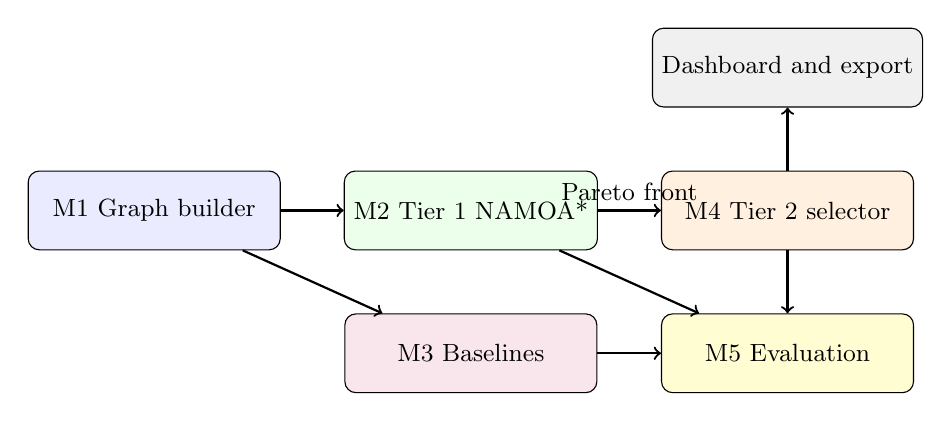
\begin{tikzpicture}[node distance=0.8cm, every node/.style={font=\small}]
  \node[draw, rounded corners, fill=blue!8, minimum width=3.2cm, minimum height=1cm] (m1)
    {M1 Graph builder};
  \node[draw, rounded corners, fill=green!8, minimum width=3.2cm, minimum height=1cm, right=of m1] (m2)
    {M2 Tier 1 NAMOA*};
  \node[draw, rounded corners, fill=orange!12, minimum width=3.2cm, minimum height=1cm, right=of m2] (m4)
    {M4 Tier 2 selector};
  \node[draw, rounded corners, fill=purple!10, minimum width=3.2cm, minimum height=1cm, below=of m2] (m3)
    {M3 Baselines};
  \node[draw, rounded corners, fill=yellow!18, minimum width=3.2cm, minimum height=1cm, below=of m4] (m5)
    {M5 Evaluation};
  \node[draw, rounded corners, fill=gray!12, minimum width=3.2cm, minimum height=1cm, above=of m4] (ops)
    {Dashboard and export};

  \draw[->, thick] (m1) -- (m2);
  \draw[->, thick] (m2) -- node[above]{Pareto front} (m4);
  \draw[->, thick] (m1) -- (m3);
  \draw[->, thick] (m2) -- (m5);
  \draw[->, thick] (m3) -- (m5);
  \draw[->, thick] (m4) -- (m5);
  \draw[->, thick] (m4) -- (ops);
\end{tikzpicture}
\caption{Review 2 architecture aligned to the implemented modules}
\label{fig:architecture}
\end{figure}

\section{Modules}
\begin{table}[H]
\centering
\caption{Implemented module responsibilities}
\label{tab:modules}
\begin{tabularx}{\textwidth}{p{0.18\textwidth}p{0.28\textwidth}X}
\toprule
\textbf{Module} & \textbf{Source file} & \textbf{Responsibility} \\
\midrule
M1 Graph builder & \texttt{module1\_graph\_builder.py} &
Builds synthetic or lattice airspace graphs, assigns distance, energy, risk and risk components to edges. \\
\addlinespace
M2 Tier 1 & \texttt{module2\_tier1\_moastar.py} &
Runs NAMOA*/multi-objective A* to generate a non-dominated route front and diagnostics. \\
\addlinespace
M3 Baselines & \texttt{module3\_baselines.py} &
Provides single-objective A*, weighted-sum A* and MOPSO comparison methods. \\
\addlinespace
M4 Tier 2 & \texttt{module4\_tier2\_payload.py} &
Validates \(\tagtuple\), derives weights, filters infeasible routes and returns a detailed selection result. \\
\addlinespace
M5 Evaluation & \texttt{module5\_evaluation.py} &
Computes hypervolume, IGD, spread, payload-alignment evidence, sweep rows and risk-component shares. \\
\bottomrule
\end{tabularx}
\end{table}

\chapter{Implementation}
\section{Graph and Cost Pipeline}
The graph builder supports deterministic synthetic graphs for offline tests and a lattice-based OSM demo path for
the Thiruvanmiyur region. Edge cost is represented as \([d,e,r]\). The current implementation includes weather,
terrain and risk hooks, but live providers have not been verified in this report. The test fixtures are hand-made or
offline-generated and should not be treated as measured field data.

\section{Tier 1 Search}
Tier 1 uses a label-setting multi-objective A* implementation. Each label carries cumulative distance, energy and
risk. A route is kept only if it is not dominated by another route to the same node. The engine records diagnostics
such as expanded labels and truncation state so that benchmark rows can flag incomplete fronts.

\section{Tier 2 Selection}
Tier 2 keeps the payload-weight formula fixed because it is the project's main contribution. The current selector
adds input validation, feasibility filtering, a detailed result object, objective ranks, point classification,
latency and JSON/CSV export. It also returns a hold advisory when weather or feasibility prevents route selection.

\section{Evaluation and Integration}
The evaluation module records method metrics and Tier 2 evidence. The Tier 2 evidence uses payload-alignment score,
selected objective ranks, non-extreme count, route diversity and latency. It does not report route-selection
``accuracy'', because there is no labelled ground-truth best route for each payload. Integration extras include
QGroundControl/Mission Planner waypoint export and a minimal Tkinter dashboard for entering tags and exporting a
selected route.

\chapter{Results and Discussion}
\section{Current Validation Status}
Table~\ref{tab:validation} lists the validation status relevant to Review 2. Numbers are limited to commands and
tests available in the repository; live services and hardware are not claimed as validated.

\begin{table}[H]
\centering
\caption{Review 2 validation status}
\label{tab:validation}
\begin{tabularx}{\textwidth}{p{0.29\textwidth}p{0.22\textwidth}X}
\toprule
\textbf{Item} & \textbf{Status} & \textbf{Evidence used in this report} \\
\midrule
Tier 2 validation and export & Implemented & Unit tests cover input validation, feasibility, selection result and export helpers. \\
\addlinespace
Evaluation metrics & Implemented & Unit tests cover metric helpers, payload-alignment score, sweep row count and risk shares. \\
\addlinespace
Mission export & Implemented & Unit tests cover QGC WPL formatting, collinear merge and altitude checks. \\
\addlinespace
Dashboard helpers & Implemented & Unit tests cover tag parsing and dashboard artifact handling. \\
\addlinespace
Live weather, OSM and DEM data & Not verified here & Requires networked run and provider checks. \\
\addlinespace
Mission Planner/QGroundControl import & Not verified here & Exporter writes a .waypoints file, but app import screenshot is still pending. \\
\addlinespace
SITL and hardware flight & Not verified here & Documented as future validation in \texttt{SITL\_NOTES.md}. \\
\bottomrule
\end{tabularx}
\end{table}

\section{Tier 2 Evidence Interpretation}
The key Review 2 claim is not that Tier 2 predicts a labelled ``correct'' path. Instead, it measures whether the
selected route aligns with the payload-derived objective preference. The evaluation records:
\begin{itemize}
  \item payload-alignment score, based on the selected route's rank on distance, energy and risk;
  \item objective ranks of the chosen route within the Pareto front;
  \item whether the chosen route is an extreme, knee, boundary or interior point;
  \item count of non-extreme selections across payload combinations;
  \item selection latency median and p95.
\end{itemize}
This evidence is better matched to the project objective than classification accuracy, because no external oracle
labels one unique best route for each payload.

\section{Limitations}
The present Review 2 report carries the following limits:
\begin{itemize}
  \item Current automated checks are offline and deterministic; real service behaviour is still unknown.
  \item Wind is modelled as a spatially uniform snapshot over the local region.
  \item Risk is a weighted exposure score, not a calibrated accident probability.
  \item Terrain and building data are sampled at graph resolution; roof-clipping edges are penalised but not yet
  hard-blocked.
  \item Battery and payload constants require final airframe calibration before field claims can be made.
  \item SITL, ground-station import and hardware flights remain future validation.
\end{itemize}

\begin{thebibliography}{99}
\bibitem{chokkalingam2026}
B. Chokkalingam and R. Ganesan, ``A hybrid Pareto optimal particle swarm optimization and reinforcement learning for
real-time UAV navigation,'' \textit{RAIRO Operations Research}, 2026. DOI: \url{https://doi.org/10.1051/ro/2025159}.

\bibitem{ren2019}
Z. Ren, J. Han, J. Feng, and Z. Zhou, ``A two-stage path planning algorithm for unmanned aerial vehicles in
urban environments,'' \textit{IEEE International Conference on Service-Oriented System Engineering}, 2019.
DOI: \url{https://doi.org/10.1109/SOSE.2019.00059}.

\bibitem{tsoutsouras2020}
V. Tsoutsouras, A. Tzes, and G. C. Karras, ``A multi-objective path planning algorithm for UAVs using particle swarm
optimization,'' arXiv:2001.02531, 2020.

\bibitem{deb2002}
K. Deb, A. Pratap, S. Agarwal, and T. Meyarivan, ``A fast and elitist multiobjective genetic algorithm: NSGA-II,''
\textit{IEEE Transactions on Evolutionary Computation}, vol. 6, no. 2, pp. 182--197, 2002.
\end{thebibliography}

\end{document}
